\documentclass[12pt]{article}
\usepackage[left=1in,top=1in,right=1in,bottom=1in]{geometry}
\usepackage[font=footnotesize]{caption}
\usepackage{parskip}
\usepackage{times}
\usepackage{graphicx}
\usepackage{mathtools}
\usepackage{gensymb}
\usepackage{placeins}

%\setlength{\parindent}{0cm}
\setlength{\parskip}{\baselineskip}


\begin{document}

	\subsubsection*{3D Rendering}
	
	So we have a right-handed coordinate system. On your computer screen, if the x-axis points right and the y-axis points up, then the z-axis points out of the screen right towards your face.
	
	Presumably all of the interesting stuff (e.g. vector fields, solenoids) will take place centered at the origin, so it'd be simpler if our viewpoint is always pointed at the origin. The locus of possible viewpoints forms a viewing sphere around the origin. (Figure 1).
	
		\begin{figure}[ht!] 
		\centering
		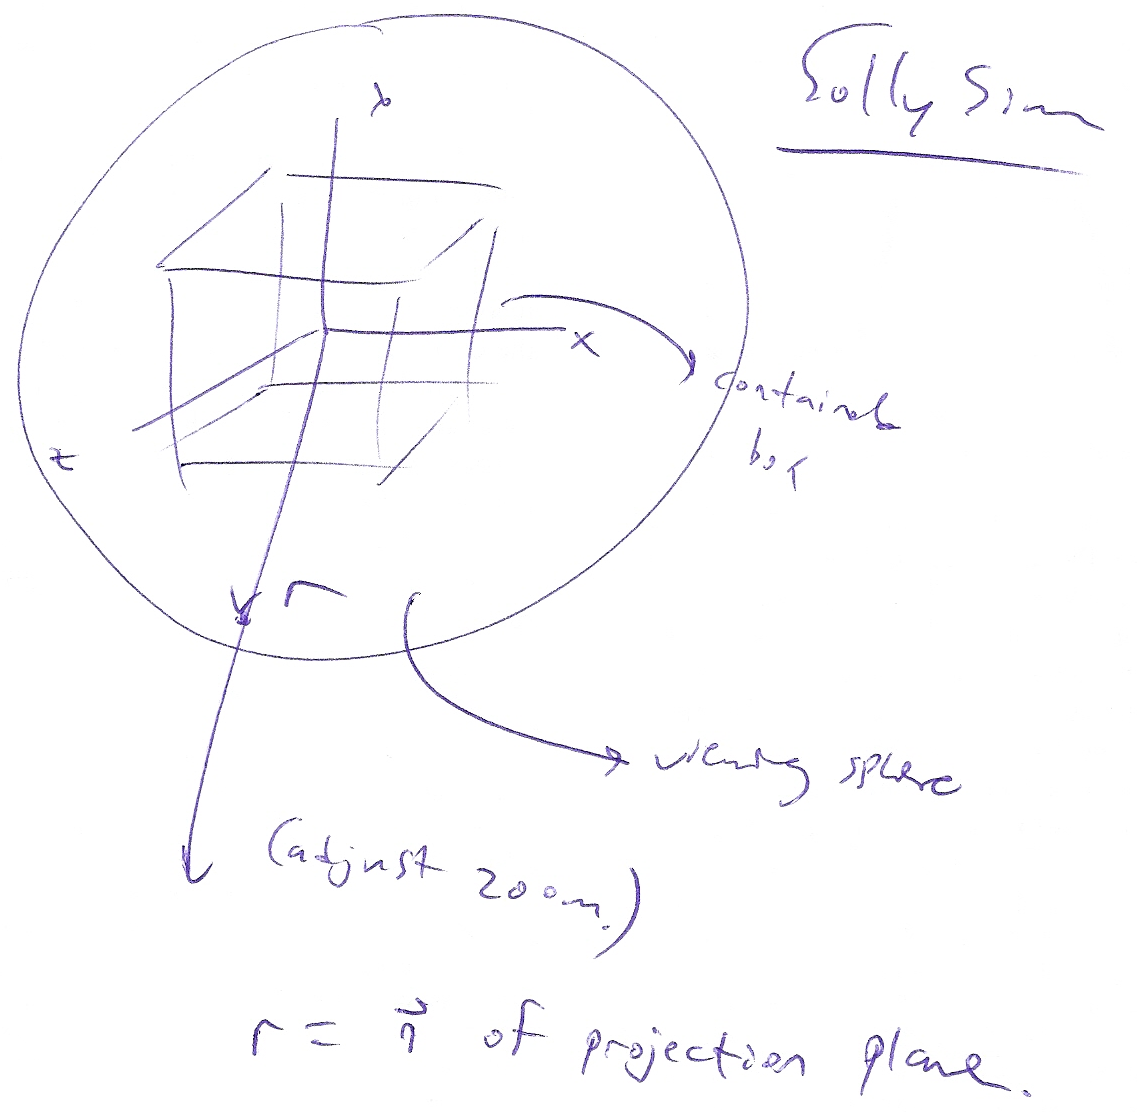
\includegraphics[width=10cm]{1.png}
		\caption{Our point of view can be anywhere on this sphere, looking in towards the origin. The image will be projected onto a plane normal to this sphere. The resulting image can be scaled afterwards to adjust zoom.} \label{im:1}		
		\end{figure}
	
	We will use ray tracing to render 3D. To properly get that perspective effect, we need a screen and a camera. The screen is a plane and the camera is a point. Let's call the position of the camera~\textbf{C}. 
	
	To avoid distortion, \textbf{C} should be right in line with the center of the screen and the origin. Let \textbf{M} be the center of the screen. Conveniently, because we're centered on the origin, the normal to the screen plane is the same as \textbf{M}. But to avoid confusion, let $\vec{n}$ be the normal to the screen. (Figure 2).

		\begin{figure}[ht!] 
		\centering
		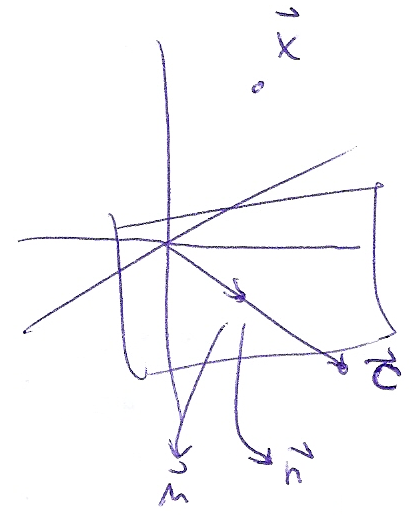
\includegraphics[width=5cm]{2.png}
		\caption{A screen and a camera looking at the origin. The arrows here denote the positions vectors of \textbf{C} and \textbf{M}. An arbitrary point \textbf{X} is also shown.} \label{im:2}		
		\end{figure}

	If we have an arbitrary point \textbf{X} in front of the screen, then our line of sight will be the line segment $\overline{\textbf{XC}}$. Where the line of sight intersects with the screen will be what our program will display on your screen.
	
	In vector form, the line of sight is:	
			$$\overrightarrow{XC} = \vec{X} + t(\vec{C}-\vec{X})$$			
	where t is some number that we don't know yet. Say this line intersects the screen at point \textbf{P}. If $\vec{P}$ is on the plane, then by definition
			$$(\vec{P} - \vec{M}) \cdot \vec{n} = 0$$
	Substituting $\overrightarrow{XC}$ for $\vec{P}$,	
			$$(\vec{X} + t(\vec{C} - \vec{X}) - \vec{M}) \cdot \vec{n} = 0$$
	Expanding,
			$$\vec{X} \cdot \vec{n} + t(\vec{C}-\vec{X}) \cdot{n} - \vec{M} \cdot \vec{n} = 0$$
	Solving for t,
			$$t(\vec{C}-\vec{X}) \cdot{n} = \vec{M} \cdot \vec{n} - \vec{X} \cdot \vec{n}$$
			$$t = \frac{\vec{M} \cdot \vec{n} - \vec{X} \cdot \vec{n}}{(\vec{C}-\vec{X}) \cdot{n}}$$
			$$t = \frac{(\vec{M} - \vec{X}) \cdot \vec{n}}{(\vec{C}-\vec{X}) \cdot{n}}$$
	Thus, the point of intersection between the $\overline{XC}$ and the screen is
			$$\vec{P} = \vec{X} + \left[\frac{(\vec{M} - \vec{X}) \cdot \vec{n}}{(\vec{C}-\vec{X}) \cdot{n}}\right](\vec{C} - \vec{X})$$
	If we have an x-axis and y-axis direction vector on the plane, then
			$$x_{s} = \vec{P} \cdot \vec{i_{s}}$$
			$$y_{s} = \vec{P} \cdot \vec{j_{s}}$$
	Where $x_{s}$ and $y_{s}$ are the x and y coordinates of the projected point on the screen, and $\vec{i_{s}}$ and $\vec{j_{s}}$ are the direction vectors for the x and y axes on the screen, respectively.

		\begin{figure}[ht!] 
		\centering
		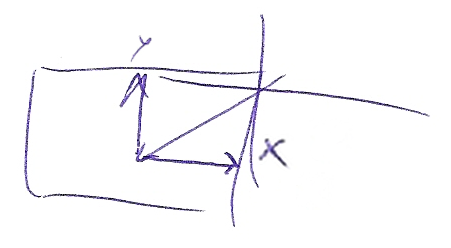
\includegraphics[width=8cm]{3.png}
		\caption{Here x denotes the $\vec{i_{s}}$ vector and y denotes the $\vec{j_{s}}$ vector} \label{im:3}		
		\end{figure}
	
	We'll later have to do a translational shift on $x_{s}$ and $y_{s}$ of (width/2, height/2) so that the point (0,0) appears at the center of the screen, but that's trivial stuff.

	\subsubsection*{Direction}
	
	We only want to render points that are behind the screen. We do this by comparing the lengths of $\overline{XP}$ and $\overline{XC}$. \textbf{X} is only behind the screen if $\overline{XP}$ is less than $\overline{XC}$. This can be checked easily with the value of t. The direction vector of the line $\overrightarrow{XC}$ has the same magnitude as the distance between \textbf{X} and \textbf{C}.
	
		1. If $t > 1$, then \textbf{X} is behind the camera and the screen. \\*
		2. If $t = 1$, then \textbf{C} is on the screen. \\*
		3. If $0 < t < 1$, then \textbf{X} is where we want it to be. \\*
		4. If $t = 0$, then \textbf{X} is on the screen. \\*
		5. If $t < 0$, then \textbf{X} is between the camera and the screen.
		
	So we want to render the point only if t is between 0 and 1.
	
	\subsubsection*{No Foreshortening}
	
	If parallel projection is desired, then set the direction vector of $\overrightarrow{XC}$ to be equal to $\vec{n}$. Thus all rays are perpendicular to the screen. In this case:
	
		1. If $t > 0$, then \textbf{X} is behind the screen. \\*
		2. If $t = 0$, then \textbf{X} is on the screen. \\*
		3. If $t < 0$, then \textbf{X} is in front of the screen.

	So we want to render the point only if t is greater than 0.

	\subsubsection*{Position}
	
	The camera should be in line with the center of the screen and the origin. Shifting the camera or screen out of line distorts the image.
	
	Moving the camera further from the screen decreases the field of view and also decreases the prominence of foreshortening. Parallel projection is equivalent to a camera at infinite distance.
	
	Moving the camera and screen system further away from the origin decreases the apparent size of objects there.

	\subsubsection*{Rotation}
	
	We want to be able to move our screen and camera so that we can view the scene from any conceivable angle. We do this by rotating $i_{s}$, $j_{s}$, the screen and the camera based on user input. Usually, one of the screen axes is recomputed from the cross product between the screen position vector and the other screen axis to maintain rigidity: This way, $i_{s}$ and $j_{s}$ are always at sharp 90 degree angles, and this angle is not susceptible to error accumulations due to rotation matrices.
	
	From Wikipedia, the rotation matrix of angle $\theta$ about a unit vector $\vec{u}$ is the following:
	

		\[R = \begin{bmatrix}
			\cos\theta + u_{x}^{2}(1-\cos\theta) & 
			u_{x}u_{y}(1-\cos\theta) - u_{z}\sin\theta & 
			u_{x}u_{z}(1-\cos\theta) + u_{y}\sin\theta \\
			
			u_{y}u_{x}(1-\cos\theta) + u_{z}\sin\theta &			
			\cos\theta + u_{y}^{2}(1-\cos\theta) &
			u_{y}u_{z}(1-\cos\theta) - u_{x}\sin\theta \\
			
						 
			u_{z}u_{x}(1-\cos\theta) - u_{y}\sin\theta & 
			u_{z}u_{y}(1-\cos\theta) + u_{x}\sin\theta &
			\cos\theta + u_{z}^{2}(1-\cos\theta) \\
			
		\end{bmatrix}\]	
		
	To maximize intuitiveness of interface, all rotations will be relative to the current location of the screen. 
	
		1. The 1-3 keys "yaw" the viewpoint, rotating about $\vec{j_{s}}$. \\*
		2. The 2-8 keys "pitch" the viewpoint, rotating about $\vec{i_{s}}$. \\*
		3. The 4-6 keys "roll" the viewpoint, rotating about $\vec{n}$.		
	
\end{document}